\section{Additional behavioral controls and auxiliary scope}
\label{app:additional-controls}

\begin{figure}[h]
    \centering
    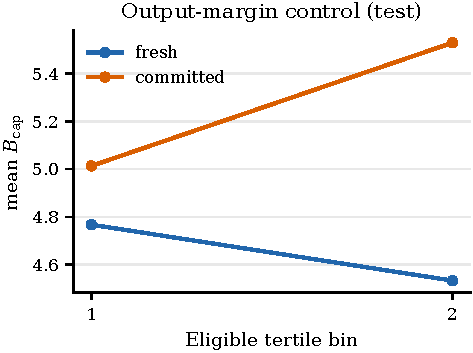
\includegraphics[width=0.58\linewidth]{figures/figureA1_output_margin_control.pdf}
    \caption{Locked output-margin control on held-out MHST/Qwen test pairs. The same-sign effect remains visible under the eligible tertile-bin fallback used by the project.}
    \label{fig:output-margin}
\end{figure}

\begin{table}[h]
    \centering
    \small
    \begin{threeparttable}
    \caption{Auxiliary scope summary. These settings are reported to bound scope, not to carry the paper.}
    \label{tab:scope}
    \begin{tabularx}{\linewidth}{>{\raggedright\arraybackslash}X c c c >{\raggedright\arraybackslash}X}
        \toprule
        Setting & Valid pairs & Mean $\DeltaBpair$ & 95\% CI & Note \\
        \midrule
        MHST / Qwen2.5-7B & 185 & 2.7784 & [2.3836, 3.1893] & Primary setting; no-conflict sanity passes \\
        MHST / Llama-3.1-8B & 39 & 0.9231 & [0.5897, 1.2827] & Same-sign but lower coverage \\
        RC-ICL / Qwen2.5-7B & 225 & 0.5244 & [0.2043, 0.8401] & Same-sign but no-conflict sanity fails ($0.70 < 0.95$) \\
        \bottomrule
    \end{tabularx}
    \end{threeparttable}
\end{table}

\begin{figure}[h]
    \centering
    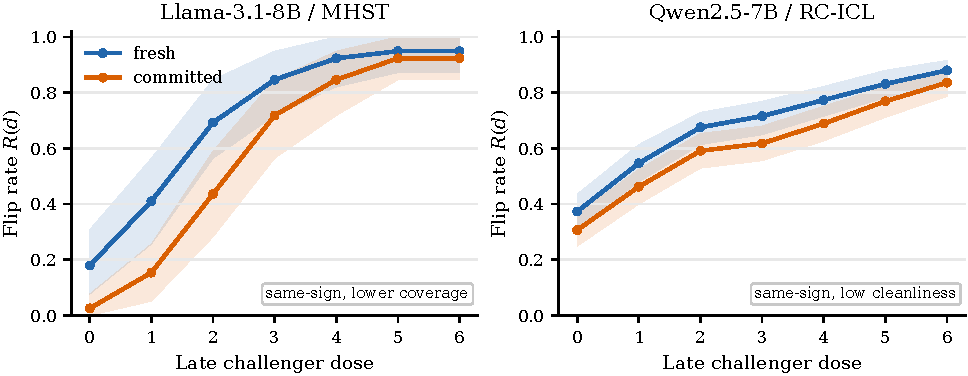
\includegraphics[width=\linewidth]{figures/figureA2_scope_curves.pdf}
    \caption{Auxiliary scope curves. The Llama MHST check is same-sign but lower-coverage. The RC-ICL check is same-sign on its main barrier summary but fails the project's cleanliness threshold, so it remains auxiliary rather than paper-central.}
    \label{app:scope}
\end{figure}
